% !Mode:: "TeX:UTF-8"
\chapter{基于时间序列预测音乐流行趋势模型}
音乐流行趋势的预测研究可以作为一个时间序列问题来研究。时间序列问题的主要特征就是(1)假设事物发展趋势会延伸到未来;(2)预测所依据的数据具有不规则性;(3)不考虑事物发展之间的因果关系。时间序列可能包含某种趋势、季节性、周期性和随机性等成分。时间序列的趋势可分为线性趋势和非线性趋势。利用回归分析可以拟合出预测趋势线。若数据元素随时间推移按线性变化,则可对时间序列拟合趋势直线;若呈现出某种非线性趋势,则需要拟合趋势曲线。由于音乐数据往往会呈现如上描述的特点,歌曲播放量的预测问题往往可以按照这些特点依次分析。除此之外,音乐播放数量的预测不单单只依赖于以往的历史数据就能分析准确的,还要考虑其他因素,比如当天是否新专辑发布等,综上,音乐流行趋势预测问题需要综合考虑多方面因素。
%%%>>>>>>>>>>>>>>>>>>>>>
\section{基于LSTM的时间序列预测音乐流行趋势模型}
\subsection{所用的算法工具}
此算法所用的语言是Python。程序编译器是Anaconda Spyder。时间序列预测问题是一类困难的预测建模问题。与回归预测建模不同,时间序列还增加了输入变量之间序列相关性的复杂性。循环神经网络是一种用于处理序列依赖性的强大神经网络。长短期记忆网络(LSTM)是一种用于深度学习的循环神经网络,LSTM适合用于处理序列特性强的数据,长期记忆性能好。本文使用Python使用LSTM算法建模预测,使用KERAS深度学习库来解决时间序列预测问题。
\subsection{研究思路}
第二章中已对LSTM的理论介绍过了,这里就不重复介绍。根据第三章中数据分析和处理的结果。以第一组数据集为例,这里输入层的“输入”就是user\_actions表和songs\_artists信息表中的数据。因为是对歌手的播放量进行预测,所以本节采用直接对每个歌手的播放量这一属性进行统计的方法,以音乐数据集中第一组含有50名歌手的数据为例,绘制并观察2015年3月1日至2015年8月30日这6个月内歌手的播放量变化趋势,并以歌手对应的歌曲每天的播放量、连续3天的播放量均值、连续3天的播放量方差作为一个时间点的样本,“滑动”构建LSTM网络的训练集。网络的构成如下: 
\begin{itemize}
    \item[(1)] {输入层包含3个神经元,这三个神经元分别代表播放量,播放均值,播放方差; }
    \item[(2)] {第一隐层是LSTM结构单元,具有35个LSTM单元;}
    \item[(3)] {第二隐层是LSTM结构单元,包含10个LSTM单元;}
    \item[(4)] {输出层包含3个神经元,这三个神经元分别代表播放量,播放均值,播放方差。}
\end{itemize}
以第一组数据集为例,随机从50名歌手抽取部分歌手的播放量、下载量、收藏量在这183天内的曲线如图~\ref{fig:5-1}~所示。

\begin{figure}[htb]
\centering

\includegraphics[width = 0.8\textwidth]{5-1.png}
\caption{部分歌手的播放量、下载量、收藏量的曲线图。绿色代表播放量,蓝色代表下载量、红色代表收藏量}
\label{fig:5-1}
% \bicaption[fig:5-1]{}{部分歌手的播放量、下载量、收藏量的曲线图。绿色代表播放量,蓝色代表下载量、红色代表收藏量}{Fig.$\!$}{The curves of number of playbacks, downloads, collections of some artists. Green line represents playbacks, blue line represents downloads and red represents collections}
\end{figure}

\subsection{预测结果}
根据前183天的播放量预测后面两个月的播放量,如图~\ref{fig:5-2}~所示,这是部分歌手的两个月播放量预测曲线和播放量真实曲线对比图。

\begin{figure}[htb]
    \centering
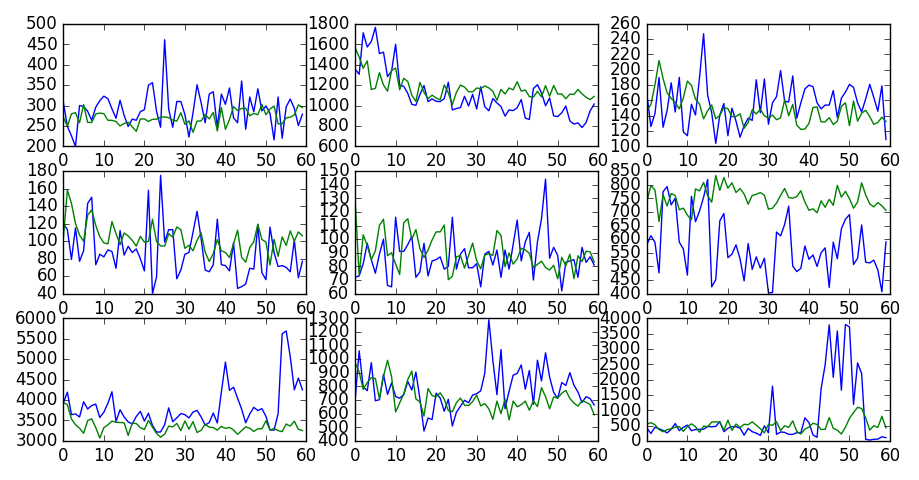
\includegraphics[width = 0.8\textwidth]{5-2.png}
\caption{部分歌手的两个月的播放量预测曲线和真实播放量的曲线对比图。蓝色代表歌手真实的播放曲线,绿色代表预测曲线}
\label{fig:5-2}
% \bicaption[fig:5-2]{}{部分歌手的两个月的播放量预测曲线和真实播放量的曲线对比图。蓝色代表歌手真实的播放曲线,绿色代表预测曲线}{Fig.$\!$}{Two months' predicting curves of playbacks of some artists comparing with their real curves. Blue line represents the artists' real playbacks curves and green line represents the prediction playbacks curves.}
\end{figure}

从对比图分析可知,大部分的歌手的预测播放量较为接近实际播放量,也存在极少数的歌手预测量偏差较大,只有第六个歌手的预测偏差较大,其他的都与实际播放量相差不大。因此,基于LSTM的时间序列预测音乐流行趋势的效果较佳。
%%%>>>>>>>>>>>>>>>>>>>>>
\section{基于ARIMA的时间序列预测音乐流行趋势模型}

\subsection{所用的算法工具}
本节算法所用的语言是R语言和python语言,编译环境为Anaconda Spyder和R x64 3.5.2。使用R语言的编辑的代码简洁灵活,可移植性强。Python拥有强大的标准库,可视化能力强。这些工具上的优势使得本节的实验达到事半功倍的效果。此外,ARIMA模型具有十分简单,只需要内生变量而不需要借助外生变量的优点,但是要求时序数据时稳定的;或者是通过差分化后是稳定的。本节将按照ARIMA模型的建模步骤实现音乐流行趋势预测。
\subsection{研究思路}
\begin{figure}[htb]
    \centering
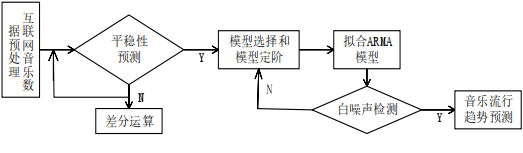
\includegraphics[width = 0.8\textwidth]{5-3.png}
\caption{ARIMA模型音乐流行趋势预测流程图}
\label{fig:5-3}
% \bicaption[fig:5-3]{}{ARIMA模型音乐流行趋势预测流程图}{Fig.$\!$}{The flow chart of music popular trend prediction based on ARIMA model}
\end{figure}
本章的ARIMA预测音乐流行趋势的流程如图~\ref{fig:5-3}~所示。从歌曲和用户两个角度进行分析建模,使用ARIMA模型。然后将两个模型的结果相融合,本节实验以音乐数据集中第一组含有50名歌手的数据为例。

一、从歌曲的角度出发

针对每首歌曲每天的播放量使用ARIMA模型进行预测后两个月的歌曲播放量,然后计算出歌手的歌曲后两个月每天的播放量。首先,获取时间序列的数据。从user\_actions表和songs\_artists信息表中统计每首歌每一天的播放量。其次,对数据集中的歌曲播放量趋势进行绘图,经过第三章对异常数据处理后,部分歌手的歌曲播放量曲线图如图~\ref{fig:5-4}~所示,观测可知为接近于平稳时间序列的非平稳时间序列,因此要先进行1阶差分运算,化为平稳时间序列,仔细分析数据集中每条记录和观察播放量曲线图可得,所有的歌曲的每日播放量都近乎是接近于平稳时间序列的非平稳时间序列,都将数据进行1阶差分运算。
 

\begin{figure}[htb]
     \centering    
    \subfigure[] {     
    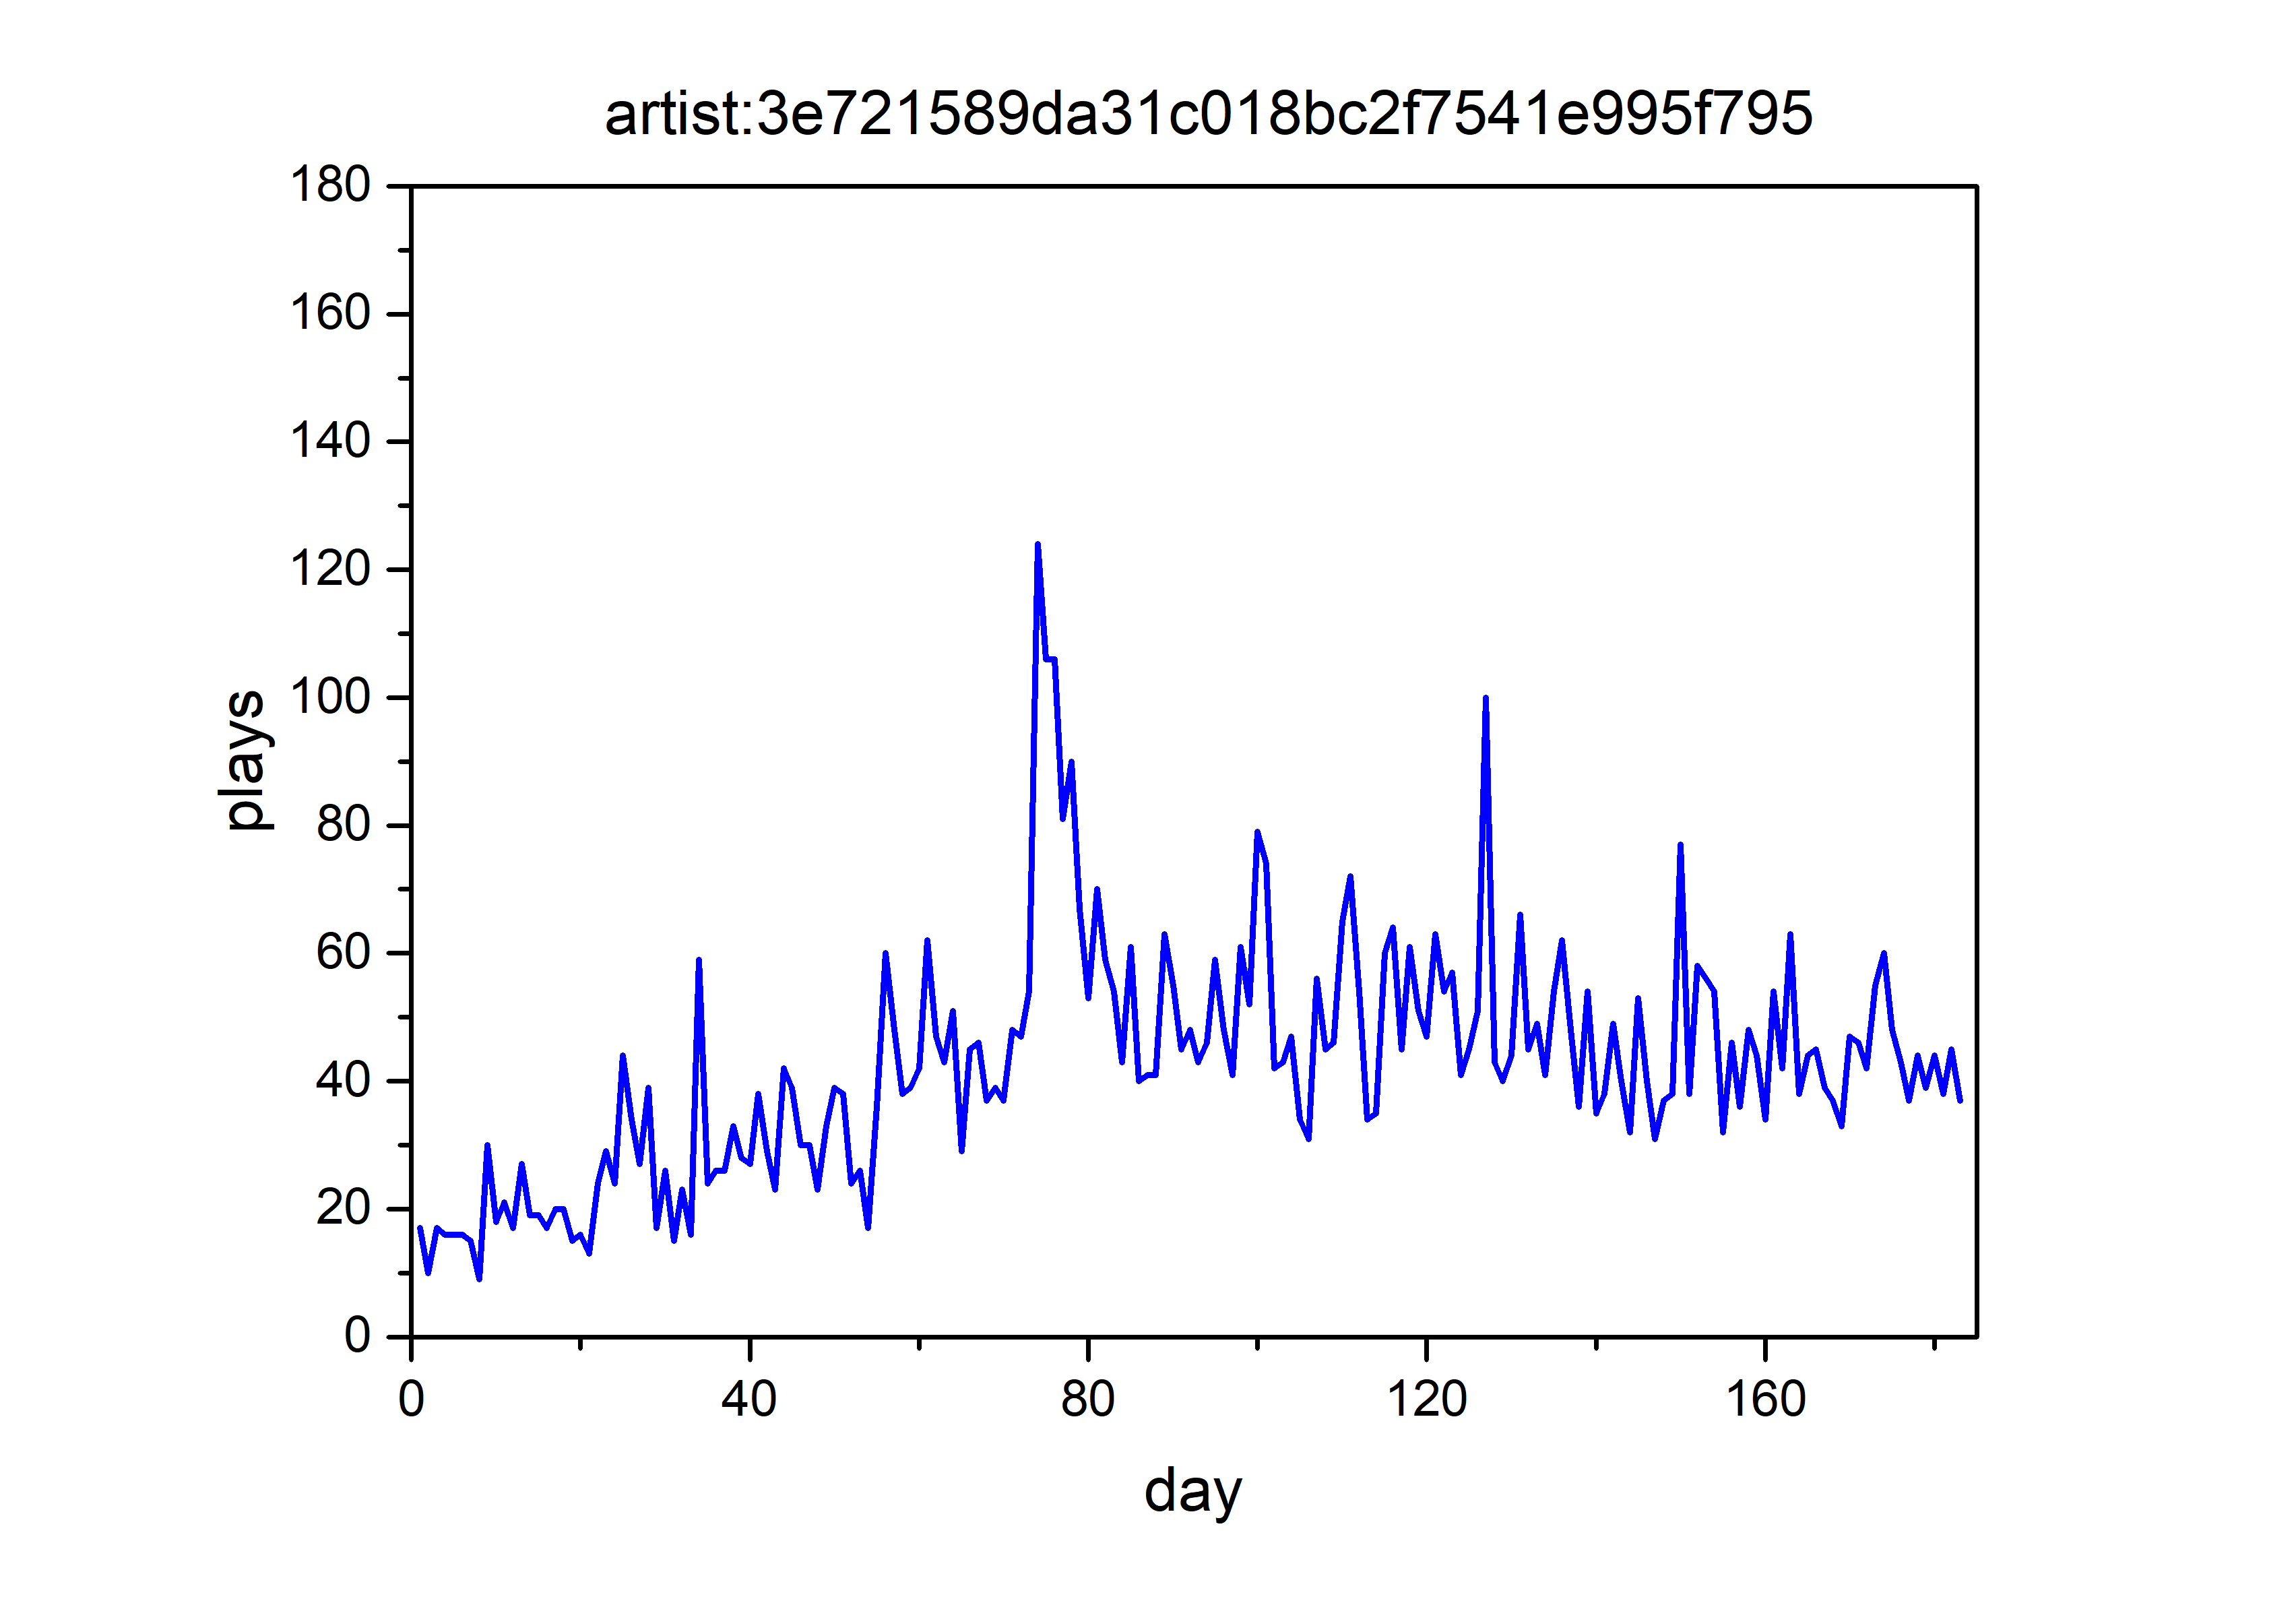
\includegraphics[width = 0.4\textwidth]{5-4-a.png}  
    }     
    \subfigure[] {     
    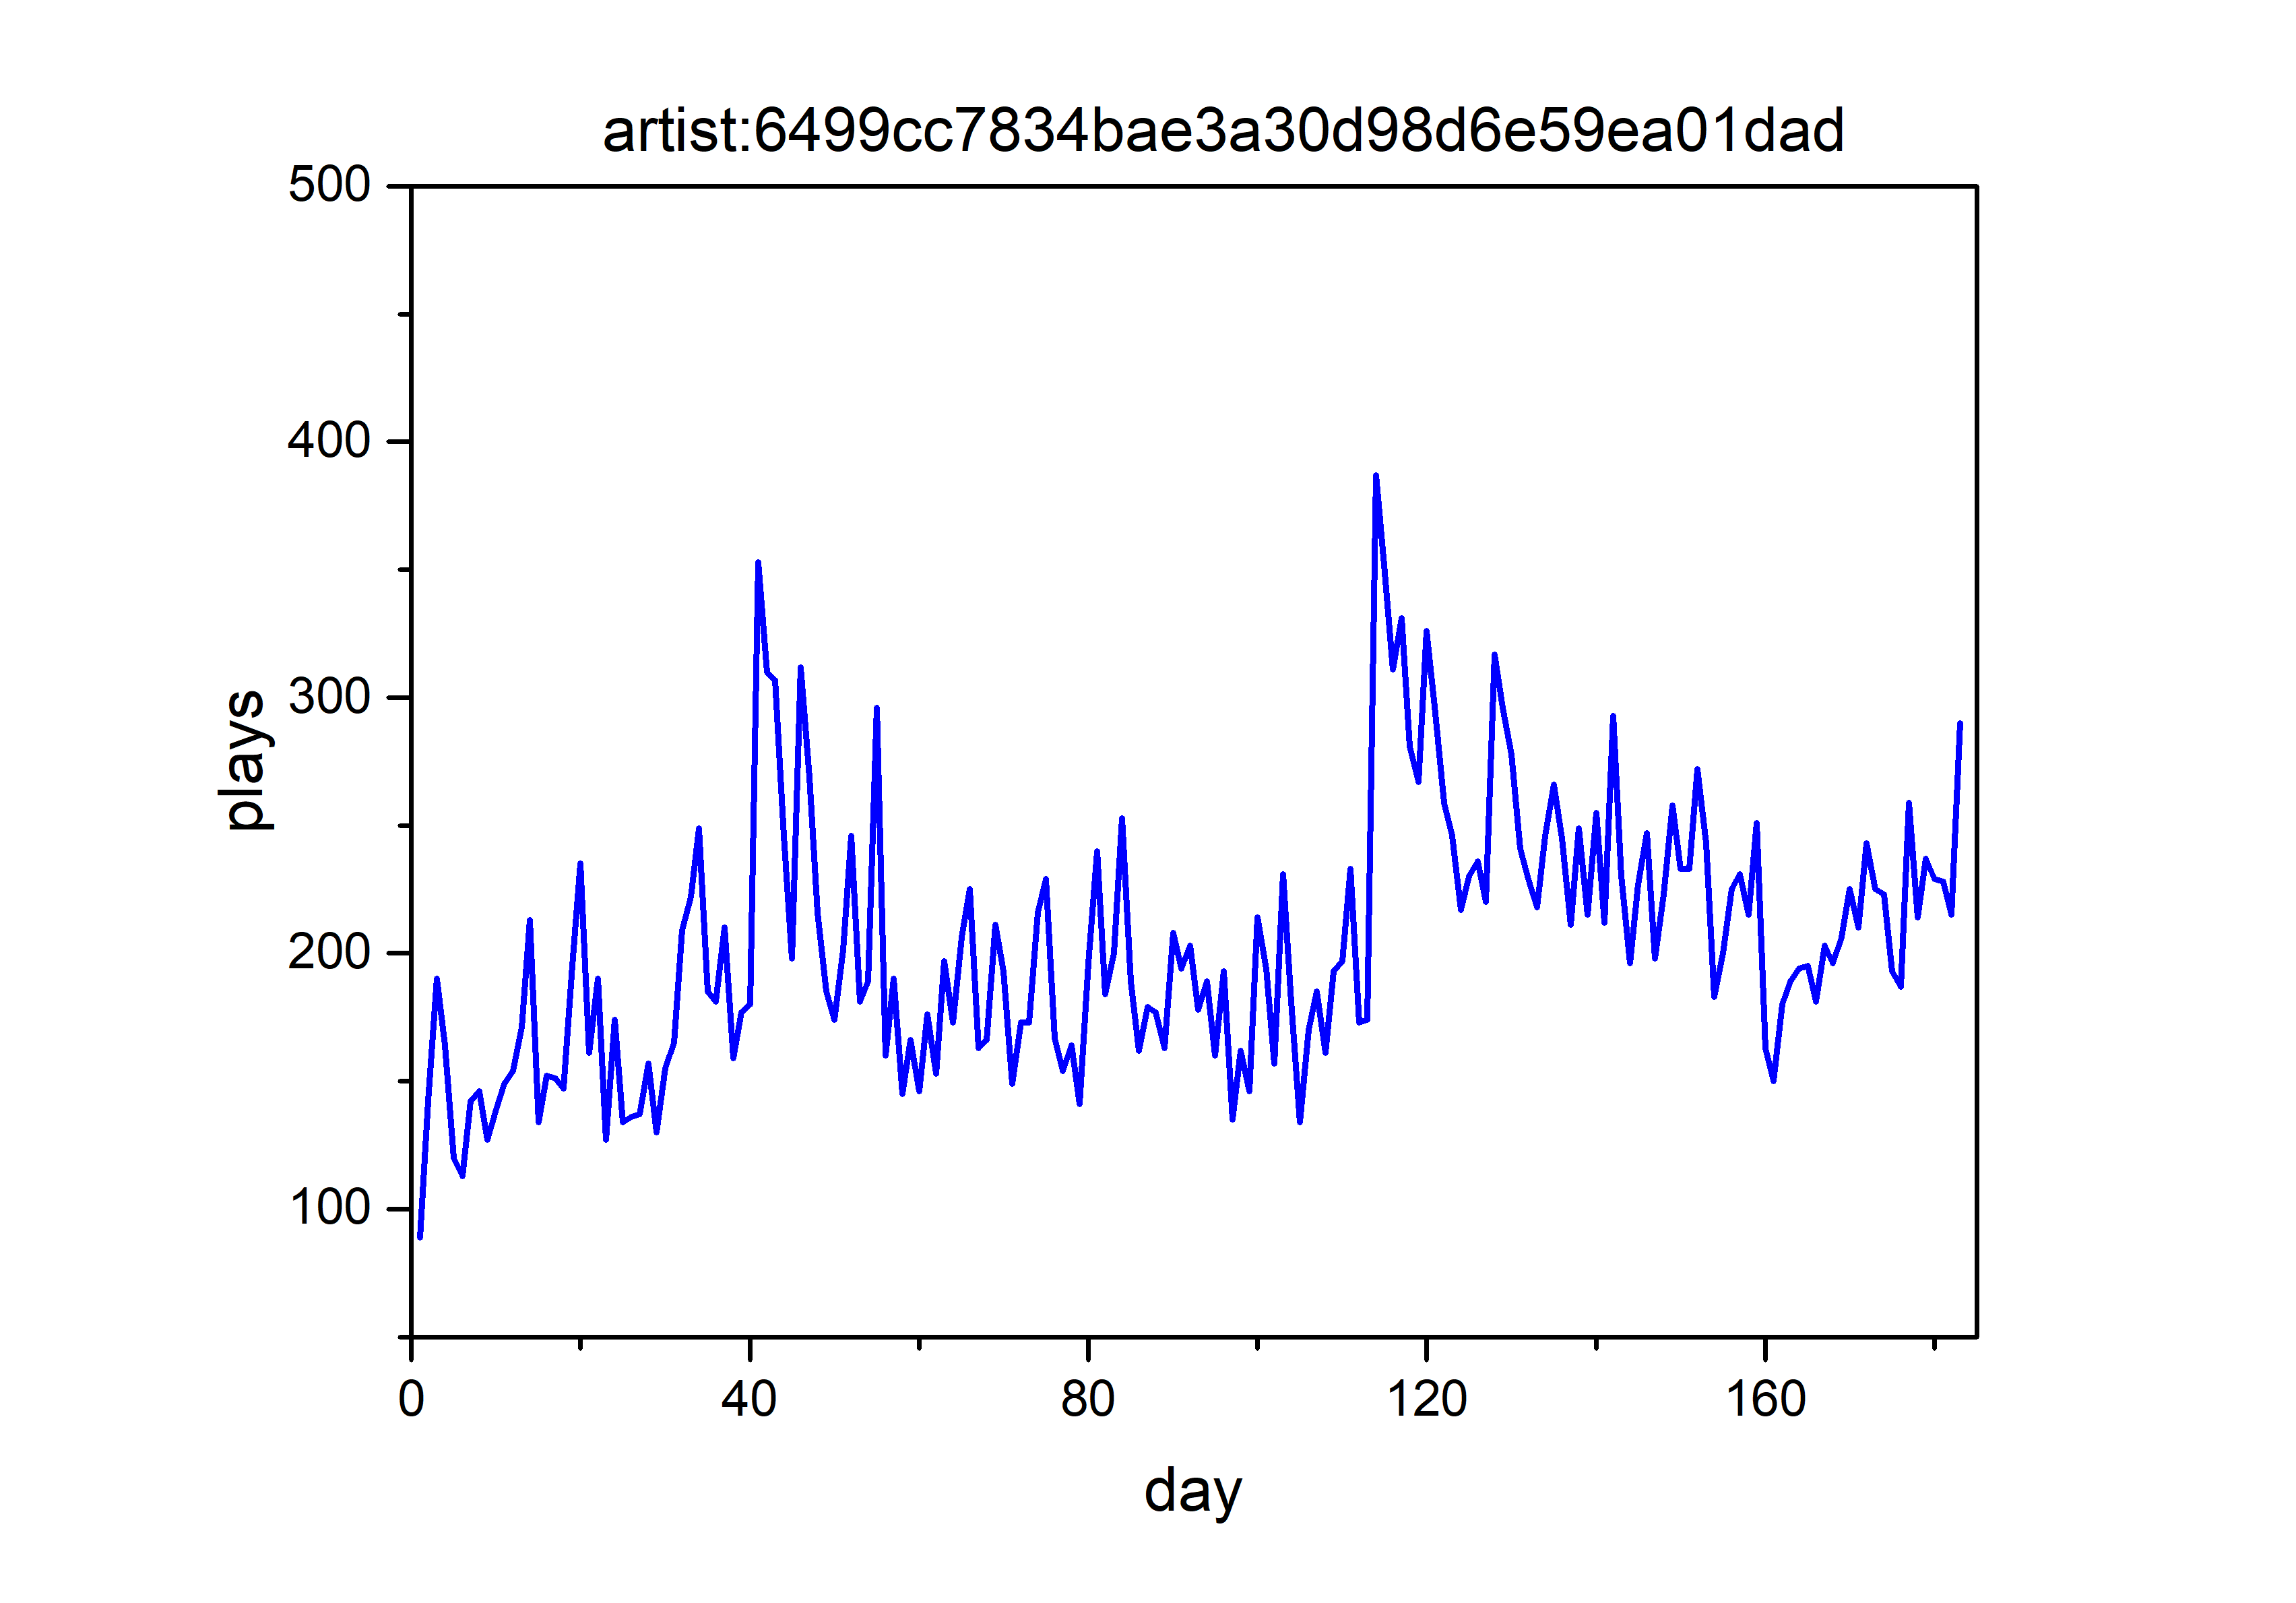
\includegraphics[width = 0.4\textwidth]{5-4-b.png}     
    }      
    \caption{a), b)为随机抽取的两个歌手的歌曲播放量曲线图 }     
    \label{fig:5-4}     
    % \bicaption[fig:5-4]{}{a),b)为随机抽取的两个歌手的歌曲播放量曲线图}{Fig.$\!$}{a),b)is the Song daily playbacks curve of two artists selected randomly}
\end{figure}

然后,再从已差分处理过的歌手的歌曲播放量中随机抽取出一个歌手编号为“1731019fbaa825714d5f8e61ad1bb7ff”的歌曲播放量数据,绘制出其自相关序列图以及偏自相关序列图如图~\ref{fig:5-5}~,~\ref{fig:5-6}~所示。自相关序列图~\ref{fig:5-5}~显示滞后1阶自相关值基本没有超过边界值,因此$p=1 $,偏自相关序列图~\ref{fig:5-6}~显示偏自相关值选5阶,$q=5 $,因此,将参数值带入拟合模型,为此歌曲构建ARIMA(1,1,5)预测音乐流行趋势模型。另外,实验过程中利用多个歌手的歌曲播放量采用了auto.arima函数产生参数值与根据序列图判断出来的参数对比实验后,auto.arima函数产生参数值较为准确,所以采用auto.arima函数来确定这些参数值。
\begin{figure}[htbp]
    \centering
    \begin{minipage}[t]{0.4\textwidth}
    \centering
    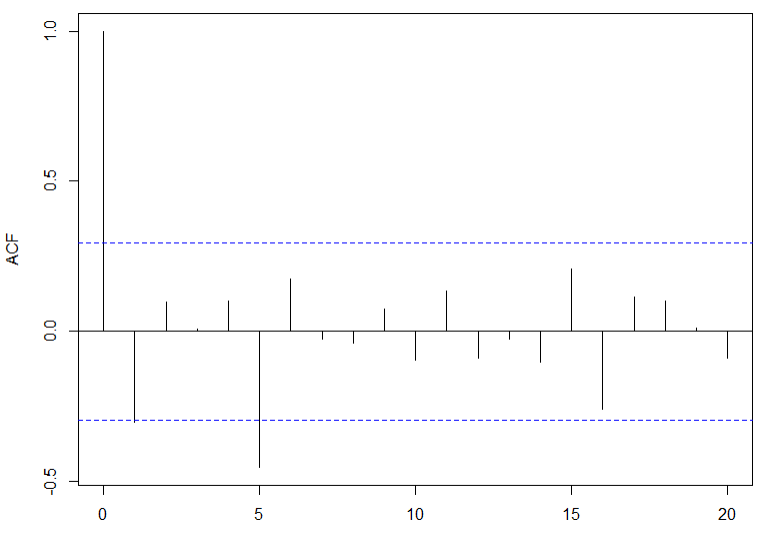
\includegraphics[width=\textwidth]{5-5.png}
    \caption{自相关序列图}
    \label{fig:5-5}
    % \bicaption[fig:5-5]{}{自相关序列图}{Fig.$\!$}{ The self-correlation coefficient diagram}
    \end{minipage}
    \centering
    \begin{minipage}[t]{0.4\textwidth}
    \centering
    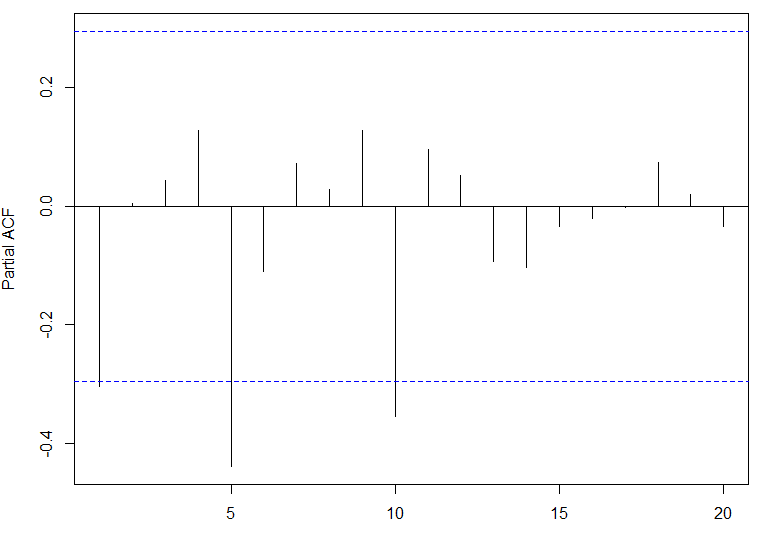
\includegraphics[width=\textwidth]{5-6.png}
    \caption{偏自相关序列图}
    \label{fig:5-6}
    % \bicaption[fig:5-6]{}{偏自相关序列图}{Fig.$\!$}{The partial correlation coefficient diagram}
    \end{minipage}
    \end{figure}

二、从用户的角度进行建模。

首先,计算出user\_actions表中每位用户六个月的总播放量、总下载量、总收藏量。其次,将相同的用户播放的相同歌曲的记录的进行合并,针对这些用户,计算出每位“用户-歌手”为主键值对的每天播放量。最后,流程如从歌曲的角度分析的一样,使用ARIMA模型预测,合并相同歌手。

三、将两种预测结果融合。

将歌曲的角度和用户的角度两种预测结果均以权重0.5相结合。

\subsection{预测结果}
通过从歌手和用户两个角度来预测歌手未来两个月的播放量,预测结果对上述个歌手“1731019fbaa825714d5f8e61ad1bb7ff”的预测播放量和实际播放量如图~\ref{fig:5-7}~所示。
\begin{figure}[htb]
    \centering
\includegraphics[width = 0.8\textwidth]{5-7.png}
\caption{预测播放量和实际播放量的曲线对比图}
\label{fig:5-7}
% \bicaption[fig:5-7]{}{预测播放量和实际播放量的曲线对比图}{Fig.$\!$}{The curve chart for predicting playbacks and actual playbacks}
\end{figure}

图中横坐标时预测的两个月的时间(9月1日至10月30日),纵坐标为歌手“1731019fbaa825714d5f8e61ad1bb7ff”的歌曲播放量,蓝色线是ARIMA模型预测的歌手歌曲播放量,红色线是实际歌手歌曲的播放量。从图中观察对比分析,预测效果较好。

将歌手“1731019fbaa825714d5f8e61ad1bb7ff”的预测播放量与实际播放量进行对比,使用平均绝对误差(MAE)进行对比,能很好地反映预测值误差的实际情况,计算公式如下:
\begin{equation}
    MAE = \frac{1}{N}\sum_{i=1}^{N}|P_i - T_i|
\end{equation}
其中,$P_i$为预测值,$T_i$为真实值。可以得到预测误差如表~\ref{tab:5-1}~所示:

\vspace{-1.5bp}
\ltfontsize{\wuhao[1.667]}
\wuhao[1.667]\begin{longtable}{cccc}%
\longbionenumcaption{}{{\wuhao 预测结果的平均绝对误差(MAE)
}\label{tab:5-1}}{Table$\!$}{}{{\wuhao Mean Absolute Error of prediction result}}{-0.5em}{3.15bp}\\
%\caption{\wuhao 中国省级行政单位一览}\\
\toprule[1.5pt] 时间 & 预测播放量& 实际播放量 & MAE  \\ \midrule[1pt]
\endfirsthead
\multicolumn{3}{r}{表~\thetable(续表)}\vspace{0.5em}\\
\toprule[1.5pt] 时间 & 预测播放量& 实际播放量 & MAE   \\ \midrule[1pt]
\endhead
\bottomrule[1.5pt]
\endfoot
2015.10.11~2015.10.15 & 479,496,478,473,478 & 469,469,469,469,475 & 0.114 \\
2015.9.6~2015.9.10 & 466,466,462,459,458 & 471,468,465,465,465 & 0.112 \\
2015.9.11~2015.9.15 & 497,505,496,478,473 & 465,469,473,473,474 & 0.167 \\
2015.9.16~2015.9.20 & 471,468,466,478,467 & 472,475,470,475,472 & 0.030 \\
2015.9.21~2015.9.25 & 466,478,467,505,496 & 471,471,468,465,470 & 0.158 \\
2015.9.26~2015.9.30 & 478,473,514,496,478 & 470,475,472,471,471 & 0.168 \\
2015.10.1~2015.10.5 & 467,505,496,478,473 & 468,465,469,469,475 & 0.158 \\
2015.10.6~2015.10.10 & 467,466,466,462,459 & 472,471,471,468,465 & 0.054 \\
2015.10.11~2015.10.15 & 479,496,478,473,478 & 469,469,469,469,475 & 0.114 \\
2015.10.16~2015.10.20 & 467,466,466,462,459 & 472,473,471,468,465 & 0.052 \\
2015.10.21~2015.10.25 & 466,478,467,496,478 & 469,475,472,471,471 & 0.086 \\
2015.10.25~2015.10.30 & 473,459,473,466,476 & 468,465,469,469,469 & 0.050 \\

\end{longtable}\normalsize
\vspace{-1em}

从上表分析可知,此歌手的歌曲真实播放量和预测播放量的平均绝对误差都不高,以求得从2015年8月1日至2015年10月30日的平均绝对误差为10.005\%。从图~\ref{fig:5-7}~和表~\ref{tab:5-1}~都能得出预测效果较佳。
%%%>>>>>>>>>>>>>>>>>>>>>
\section{实验结果总评估分析}
根据上文第四章写到评估指标进行评估,将输出两个模型的预测结果代入评估指标的代码中进行计算$F$值。两个时间序列预测模型以第一组音乐数据集为例进行实验,计算得基于LSTM的时间序列音乐流行趋势预测模型的$F$值为26504.734579438790067。测试计算得基于ARIMA的时间序列音乐流行趋势预测模型的$F$值为28707.588970085433219。相对比来说,基于ARIMA的时间序列音乐流行趋势预测模型的预测效果优于基于LSTM的时间序列音乐流行趋势预测模型。

第二组数据使用相同的方法进行实验验证两个时间序列预测模型,得出实验结果。本文实验结果如下~\ref{tab:5-2}~所示和图~\ref{fig:5-8}~所示,结合第四章利用随机森林算法预测音乐流行趋势模型和爆增型歌曲衰减模型组合预测的结果,相对比于LSTM时间序列预测模型和ARIMA时间序列预测模型效果更佳。总体而言,四个预测模型的预测效果都很不错,达到预期的预测目标。

\begin{table}[htbp]
    \bicaption[tab:5-2]{}{四个模型评估指标F值结果}{Table$\!$}{The evaluation indicator F value of the four models}
    \vspace{0.5em}\centering\wuhao
    \begin{tabular}{ccccc}
    \toprule[1.5pt]
    数据集 & RandomForest& RF+ESAM & LSTM & ARIMA\\
    \midrule[1pt]
    第一组 & 29391 & 43812 & 1.79 & 26504\\
    第二组 & 54208 & 63198 &49098 &53147\\
    \bottomrule[1.5pt]
    \end{tabular}
\end{table}

\begin{figure}[htb]
    \centering
\includegraphics[width = 0.5\textwidth]{5-8.png}
\caption{四个模型评估指标F值}
\label{fig:5-8}
% \bicaption[fig:5-8]{}{四个模型评估指标F值}{Fig.$\!$}{The evaluation indicator F value of the four models}
\end{figure}


\section{本章小结}
本章首先分析互联网音乐数据的时间序列的特性,构建一种基于长短期记忆网络时间序列预测流行音乐趋势模型和构建基于差分自回归移动平均法时间序列预测音乐流行趋势模型。利用通过实验测试、验证两个时间序列预测模型的效果,且评估对比分析预测能力。与第四章构建的随机森林预测音乐流行趋势预测模型和爆增型歌曲衰减模型进行对比,得出随机森林预测音乐流行趋势模型和爆增型歌曲的衰减模型的组合预测模型预测效果相对较好的最终实验结论,此结论达到了预期的实验目标。